\begin{figure}[htpb]
\centering
\makebox[\textwidth]{%
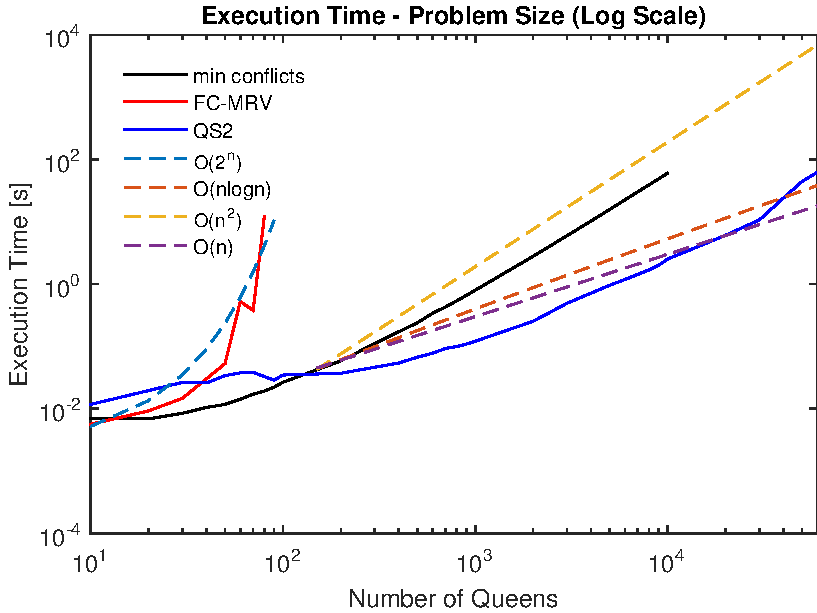
\includegraphics[width=0.8\textwidth, angle = 0, trim = 0mm 0mm 0mm 0mm,clip=true]{images/execution-time.pdf}}
\caption{Real execution time as a function of $n$ from the data of Table \ref{table:execution-time}. To reveal the scaling of each algorithm's time complexity, we also draw representative exponential and polynomial functions.}
\label{fig:execution-time}
% Place the label just after the caption to make the link work
\end{figure} % table makes a floating object with a title